\begin{frame}{Demo}{}
	Skift over til terminal\\
	Start\\
	Forklar, antal payloads, kompleksitet og tidsplanens laengde\\
	Vis gantt chart imens at vi venter (gem et saadan at det ikke overskrives undervejs)\\
	Hop tilbage igen og vis vi blev faerdig
\end{frame}

% Output intro
\begin{frame}{Output}{}
	Output Files
	\begin{itemize}
		\item Raw schedule / trace
		\item Gantt chart
		\item SMC query results
		\item Adjusted CORA model
		\item Adjusted SMC model
	\end{itemize}
\end{frame}

% Output 1
\begin{frame}[fragile]{Output}{Query 4.8}
	% query 4.8 - den der viser om vi havde strom nok til sidst - men ikke hvor meget
	\begin{equation*}
		Pr\; [<=ScheduleLength] \; (<>\; b\ +\ a\ <\ C\ *\ (ThresholdPercentage\ /\ 100)
	\end{equation*}
	% Result
	\begin{lstlisting}
		Verifying formula 1 at line 1
		-- Throughput: 155813 states/sec, Load: 389 runs
		-- Throughput: 411877 states/sec, Load: 385 runs
		-- Throughput: 413986 states/sec, Load: 374 runs
		-- Throughput: 414674 states/sec, Load: 362 runs
		-- Formula is satisfied.
		(36 runs) Pr(<> ...) in [0,0.0973938]
		with confidence 0.95.
	\end{lstlisting}
	\pause
	\begin{equation*}
		simulate\ 100 \; [<=\ ScheduleLength]\; \{ a,\ b\}
	\end{equation*}
\end{frame}

% Output 1.1 - query 4.11
\begin{frame}{Output}{Query 4.11}
	\begin{equation*}
		simulate\ 100 \; [<=\ ScheduleLength]\; \{ a,\ b\}
	\end{equation*}
	\begin{figure}
		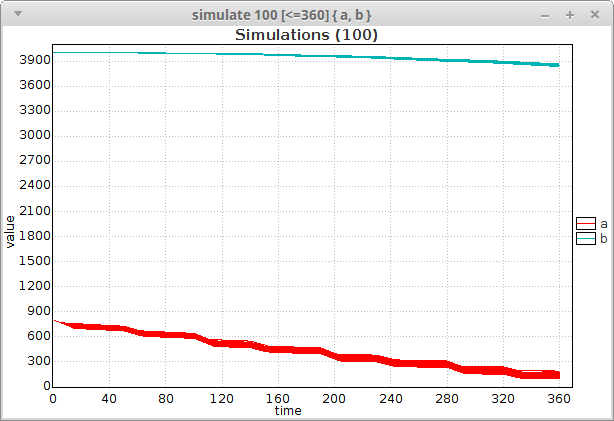
\includegraphics[width=0.60\textwidth]{graphics/ab.png}
		\end{figure}
\end{frame}

% Output 2
\begin{frame}[fragile]{Output}{Query 4.9}
	% query 4.9 - 
	\begin{equation*}
Pr\; [<=ScheduleLength] \; (<> \ skips \ !=\ 0)
	\end{equation*}
	% Result
	\begin{lstlisting}
Verifying formula 2 at line 2
-- Throughput: 64 states/sec, Load: 389 runs
-- Throughput: 386904 states/sec, Load: 389 runs
-- Throughput: 428461 states/sec, Load: 379 runs
-- Throughput: 427479 states/sec, Load: 367 runs
-- Throughput: 424452 states/sec, Load: 355 runs
-- Formula is satisfied.
(36 runs) Pr(<> ...) in [0,0.0973938]
with confidence 0.95.
	\end{lstlisting}
	\pause
	\begin{equation*}
		simulate\ 100 \; [<=ScheduleLength] \; \{active, \; Processor.Running\}
	\end{equation*}
\end{frame}

% Output 3
\begin{frame}[fragile]{Output}{Query 4.10}
	% query 4.10
	\begin{equation*}
		simulate\ 100 \; [<=ScheduleLength] \; \{active, \; Processor.Running\}
	\end{equation*}
	% Result
	\begin{lstlisting}
active:
[0]: (0,-1) (0.09,4) (13.828,4) (13.918,-1) ...
Processor.Running:
[0]: (0, 0) (0.09,1) (13.828,1) (13.918, 0) ...
	\end{lstlisting}
\end{frame}

% Output 3.1
\begin{frame}{Output}{Query 4.10}
	\begin{equation*}
		simulate\ 1 \; [<=ScheduleLength] \; \{active, \; Processor.Running\}
	\end{equation*}
	\begin{figure} % -1 og -2 IKKE 0 og 1 for .Running
		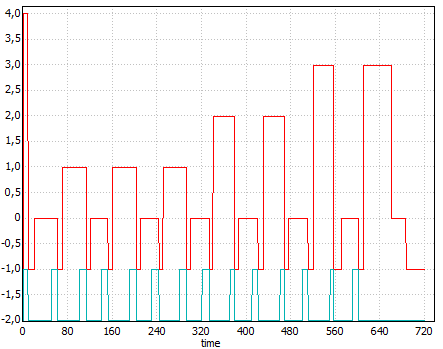
\includegraphics[width=0.45\textwidth]{graphics/activeprocessor.png}
		\end{figure}
\end{frame}

% Reflection 1 - batteri
\begin{frame}{Reflection}{Battery considerations}
	The battery is not a concern
	\begin{block}{Personal meeting with GomSpace, Lars Alminde}
		Not as important, more focus on clusters of satellites
	\end{block}
	Reasons:
	\begin{itemize}
		\item Greater battery capacity
		\item More efficient solar panels
	\end{itemize}
\end{frame}

% Reflection 2 - Robusthed
\begin{frame}{Reflection}{Robustness}
	Minimal functionality
	\begin{itemize}
		\item Varying time on payloads
	\end{itemize}
	Wanted functionality
	\begin{itemize}
		\item Randomly forced reboots
		\item Lessen the efficiently of the solar panels
		\item Payloads that takes longer than expected
	\end{itemize}
\end{frame}
